% !TEX TS-program = xelatex
% !TEX encoding = UTF-8 Unicode
% !Mode:: "TeX:UTF-8"

\documentclass{resume}
\usepackage{zh_CN-Adobefonts_external} % Simplified Chinese Support using external fonts (./fonts/zh_CN-Adobe/)
%\usepackage{zh_CN-Adobefonts_internal} % Simplified Chinese Support using system fonts
\usepackage{linespacing_fix} % disable extra space before next section
\usepackage{cite}
\usepackage{graphicx} % import graphicx, display images
\usepackage{tabularx} % import tabularx, use tables 
\usepackage{makecell}

\begin{document}
\pagenumbering{gobble} % suppress displaying page number

% \firstname{Roy}
% \familyname{Shang}
%\name{尚祚彦}
%\title{Resum\'{e}}
% \address{紫东路18号}{210046, 南京}
%\phone{(+86) 13913834668}
%\email{shangzuoyan@hotmail.com}
%\homepage{homepage (optional)}



%\maketitle

\begin{table}[!ht]
\flushleft
\begin{tabular}{lc}
\begin{minipage}{0.20\columnwidth}
    \flushleft
    {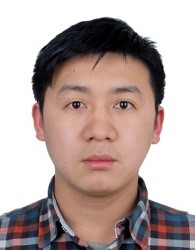
\includegraphics[width=0.8\textwidth]{./images/00.jpg}}
\end{minipage}& \begin{minipage}{.76\textwidth}\raggedright
  \pinfo{尚祚彦 | Roy(Zuoyan)Shang}{1981/01/26,南京}\leavevmode\\
  \wwwinfo{(+86) 13913834668}{shangzuoyan@hotmail.com}{https://shangzuoyan.github.io}
  \end{minipage}
\end{tabular}
\end{table}

% 00::Avatar
%\begin{figure}[htbp]
%      \flushleft
%      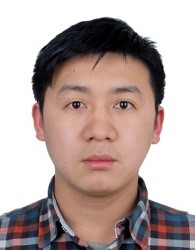
\includegraphics{./images/00.jpg}
%\end{figure}

 % \begin{flushright}
 % \email{shangzuoyan@hotmail.com}\leavevmode\newline
 % \homepage{https://shangzuoyan.github.io/}
 % \end{flushright}
%  \begin{flushright}
%  {(+86) 13913834668}\leavevmode\newline
%  {shangzuoyan@hotmail.com}\leavevmode\newline
%  {https://shangzuoyan.github.io/}\leavevmode\newline
%  \end{flushright}

%\name{尚祚彦}
%\phone[mobile]{(+86) 13913834668}
%\email{shangzuoyan@hotmail.com}
%\url{https://shangzuoyan.github.io/}
% {E-mail}{mobilephone}{homepage}
% be careful of _ in emaill address
% \contactInfo{(+86) 13913834668}{shangzuoyan@hotmail.com}{软件工程师}{GitHub @shangzuoyan}
% {E-mail}{mobilephone}
% keep the last empty braces!
% \contactInfo{shangzuoyan@hotmail.com}{(+86) 13913834668}{}



 
\section{自我评价 | Self-assessment}
熟练运用C/C++/C\#,Java,Python语言;\newline
熟悉L4微内核(SeL4/L4Re)以及QNX/HelenOS等微内核操作系统;\newline
熟悉Hypervisor虚拟化和LXC容器;\newline
熟悉Linux/Android和主流 RTOS;\newline
熟悉TCP/IP族协议,网络编程和精通设计模式;\newline
具有良好的系统架构设计能力和嵌入式系统的程序开发经验;\newline
较强的表达能力,职业级英语能力,有境外工作经验;\newline
为人诚恳,工作踏实,有较强的学习能力和合作精神;\newline
健康,开朗,有责任心。\newline
\textbf{现任职于中汽创智。}
\spaceline{}

% \section{\faGraduationCap\ 教育背景}
\section{教育 | Education}
\datedsubsection{\textbf{南京师范大学},地图学与地理信息系统|电子信息科学类,\textit{理学硕士}}{\textbf{2006.09 - 2009.06}}
\textbf{Cartography and Geographic Information Systems (Master of Science)}\newline
School of Geographical Sciences, \textbf{Nanjing Normal University (NJNU)}
\datedsubsection{\textbf{江苏大学},工业设计工程|机械电子类,\textit{工学学士}}{\textbf{1999.09 - 2003.07}}
\textbf{Industrial Design Engineering (Bachelor of Engineering)}\newline
School of Mechanical Engineering, \textbf{Jiangsu University (JSU)}
\spaceline{}

% \section{\faCogs\ IT 技能}
\section{技能 | Skills}
% increase linespacing [parsep=0.5ex]
\begin{itemize}[parsep=0.2ex]
  \item \textbf{编程语言}: C, C++, C\#, Java, Python, Shell
  \item \textbf{操作系统}: Linux/Redhat, SeL4/L4Re/HelenOS, FreeRTOS/RT-Thread/Nucleus/QNX
  \item \textbf{关键词}: GDB(Gef)/Lauterbach Trace32/ARM/RSIC-V/QEMU/Gem5
\end{itemize}

% \end{itemize}
\spaceline{}

\section{工作经历 | Work Experience}
% E:1============================================================
\datedsubsection{\textbf{中汽创智科技有限公司[CAIC]}, 基础软件部经理 / 操作系统专家}{\textbf{2021.06-至今}}
\xblock{2021.06-至今}{基础软件部经理 / 操作系统专家}{中汽创智科技有限公司[CAIC]}{智能网联事业部 / 基础软件部}
\begin{itemize}
  \item 全面负责基础软件开发部操作系统的设计研发工作。包括:\newline
 CAIC OS / CAIC Hybrid OS / CAIC Hypervisor / CAIC Hypervisor Light等产品线的设计研发工作。\newline
 NXP i.MX8QM / TI TDA4 / MTK8675 平台适配工作。
  \item 部分联合研发项目:\newline
  负责Siemens / Mentor Graphics Nucleus操作系统合作项目的系统重构设计研发以及认证工作;\newline
  负责中瓴智行虚拟化系统Raite Hypervisor合作项目的系统设计研发工作;\newline
  负责Renesas RH850/U2A/U2B的轻量级虚拟化系统项目的系统设计研发以及认证工作;\newline
  负责车身控制域基于轻量级虚拟化方案上的Zonal架构AUTOSAR CP系统;\newline
  负责地平线机器人J3/J5辅助自动驾驶操作系统合作项目的系统设计研发工作。 
\end{itemize}
\spaceline{}

% E:2============================================================
\datedsubsection{\textbf{富智康集团(南京)通讯有限公司 | FIH Communications},专理课长}{\textbf{2017.10-2021.01}}
\xblock{2006.07-2009.05}{研究生}{虚拟地理环境重点实验室[VGEKL]}{南京师范大学 / 地理科学学院}
\begin{itemize}
  \item \textbf{全面负责Sharp(SG1/HD1/VGO/VG2)以及Nokia(ROO/TAS)项目的系统设计研发以及认证工作。}\newline
精通WLAN/Bluetooth/FM/GNSS,NFC/Felica,IR等子系统及模块;\newline
参与苹果ICAR Connectivity交互场景研发;\newline
参与拜腾智慧座舱联合研发工作。
  \item \textbf{部分外包业务:}\newline
负责Vivo Khronos项目的无线通信相关子系统的设计研发以及认证工作;\newline
负责Mi D1S OTA项目的无线通信相关子系统的设计研发工作;\newline
负责Mi J15s项目的无线通信相关子系统的设计研发以及认证工作;\newline
负责LG DH0项目的无线通信相关子系统的设计研发以及认证工作。
\end{itemize}
\spaceline{}

% E:3============================================================
\datedsubsection{\textbf{江苏润和软件股份有限公司 | HopeRun},智能终端事业本部,终端OS业务条线 技术总监}{\textbf{2016.01-2017.10}}
\xblock{2006.07-2009.05}{研究生}{虚拟地理环境重点实验室[VGEKL]}{南京师范大学 / 地理科学学院}
\begin{itemize}
  \item \textbf{承接Huawei中央软件院欧拉实验室AtelierOS项目:}
AtelierOS是基于L4微内核的虚拟容器,其上可部署运行多个操作系统并进行无缝切换。
负责系统整体架构设计和实现,适配Huawei Mate系列的演进。
  \item \textbf{承接Huawei终端公司Texas AT&T项目:}
基于Qualcomm MSM8939平台,项目技术负责人,负责系统Bringup,认证工作以及问题跟踪。 
  \item \textbf{承接Huawei终端公司VR项目:}
负责项目的系统架构和设计,负责关键子系统的开发和编码工作。
基于重构gSOAP的OnVIF服务,基于libevent的进程间通信服务,以及基于Sqlite的DAL封装。
  \item \textbf{承接ClouderSemi公司Smart Watch Turnkey项目:}
负责项目的系统架构和设计,负责基于蓝牙的系统框架开发和编码工作。
基于Bluetooth LE的信令交互私有协议,基于Bluetooth RF-COMM的传输服务,以及Bluetooth HFP/A2DP的音频服务。
\end{itemize}
\spaceline{}

% E:4============================================================
\datedsubsection{\textbf{宇龙计算机通信科技(深圳)有限公司},南京研究所-第52部,主任软件工程师}{\textbf{2013.05-2016.01}}
\xblock{2006.07-2009.05}{研究生}{虚拟地理环境重点实验室[VGEKL]}{南京师范大学 / 地理科学学院}
酷派海外市场产品研发\newline
主要负责Connectivity相关模块WLAN/BT/FM Combo(Integrated)WCN3660/WCN3620/WCN3620B/WCN3610芯片的Bringup,相关模块维护,认证测试(WFA/BQB, BT-IOT等)的管控,海外运营商相关需求的沟通,以及海外在线测试问题的快速解决。

[GNSS] WTR1605L/WTR4905 Transceiver,SKY65611-11 PA(eLNA)芯片的配置(此工作包含在RF Bringup工作中),解决AGPS测试以及SUPL1.1/2.0认证测试中的问题。\newline
[NFC] NXP PN544/PN547芯片的Bringup,驱动调试,NFC协议栈升级,SmartCard方案集成,EMVCo2.3.3认证,支持VISA/MASTERCARD/AMEX支付功能。\newline
[IR] ABOV MC96FR116CU芯片的Bringup,驱动调试工作。\newline
完成TMO运营商新需求的开发工作,包括DeviceReporting,HW Encyption,Anti-theft Feature等。\newline
\newline
目前涉及相关平台如下:\newline
MSM8926(Vodafone Smart 4 Max)/MSM8916(Panasonic ELUGA L 4G)/MSM8909(中国移动Y75)/MSM8939(奇酷)等。\newline
\spaceline{}

% E:5============================================================
\datedsubsection{\textbf{信源通科技有限公司 / },南京研究所-软件部,资深软件工程师/软件部副经理}{\textbf{2009.10-2013.05}}
\xblock{2006.07-2009.05}{研究生}{虚拟地理环境重点实验室[VGEKL]}{南京师范大学 / 地理科学学院}
[高通AMSS8960平台]G6611/G3617项目 / [高通AMSS8625平台]QRD-G2616/G3616/G3617项目:主要负责Modem侧软件,承担Android Framework/RIL、QCRIL层Telephony相关代码实现。

[高通AMSS7627平台]F3610/F3611项目:主要负责Modem侧软件,负责Android Framework/RIL、QCRIL层相关代码实现,负责IOT Level2测试(美国福沃斯诺西网络实验室)。

[高通QSC6085平台]CDMA 1x EVDO M600项目:(驻美1年)主要负责MMS、WAP浏览器、WWW(Full HTML)浏览器 模块,负责MMS/WAP IOT测试(美国福沃斯摩托罗拉网络实验室),与PCD,UMX以及US Cellular讨论功能需求和技术支持事宜。基于高通QSC6085平台。

[高通QSC6055平台]CDMA 1x WMDP项目:主要负责自动语音识别[ASR](科大讯飞iFlyTek/VoiceSignal Tech)和重力传感器[G-Sensor]应用模块,参展CES2010和亚洲电信展。

[高通QSC6270平台]GSM/WCDMA WA01/WA02/ WA02(DSDS)/W399/W599/ W599(DSDS)/E7610/E7620项目:
承担底层驱动工作,包括:FLASH驱动(Micron/Hynix)、LCD/MDP驱动(松瑞Sunrise/信利Truly等,LCM驱动IC包括TM2.0 3.55 ILI9341 9225 9225G HX8340B 8347D)、T9键盘/QWERTY键盘驱动以及HALL器件翻盖器件驱动的调试以及GSDI双卡支持的底层实现工作;承担OEM接口封装层以及应用层的工作;负责短信(GSM 03.38/03.40/07.05)、彩信(TS23.140/OMA)、STK(GSM 11.14)、SIM卡(TS 31.102)、蓝牙、Brew JavaVM、WWW(Full HTML)浏览器、多媒体和输入法模块。

[高通MDM6085平台]CDMA 1x EVDO D2/D3/D5数据卡项目:主要负责下位机AT命令和上位机同步及拨号软件的开发调试任务。
\spaceline{}

% E:6============================================================
\datedsubsection{\textbf{虚拟地理环境重点实验室[VGEKL]},南京师范大学 / 地理科学学院,研究生}{\textbf{2006.07-2009.05}}
\xblock{2006.07-2009.05}{研究生}{虚拟地理环境重点实验室[VGEKL]}{南京师范大学 / 地理科学学院}
基于非流形理论的地下空间实体三维GIS关键技术研究 		2007年11月 – 2009年05月
项目编号:2007AA12Z236 [国家863项目]
从事三维GIS框架建设(OSGi RCP框架)、空间数据索引(通用搜索树GiST、空间索引库Space Index Library、混合索引OR-树的算法实现和应用)、数据可视化方面(Open Inventor, IRRLicht, OSG, Coin3D)的研究,负责原型系统的开发任务。

GIS矢量数据产品版权保护的关键技术研究				2006年10月 – 2007年03月
项目编号:2006AA12Z222 [国家863项目]
工作内容:从事伪随机序列密钥掩码(最大长度线性移位寄存器m序列,M序列,Golden序列以及混沌序列),水印嵌入和提取,小波分解与重构方面的研究,对高维空间数据进行水印嵌入,以达到保护空间数据的目的,参与完成原型系统的开发任务。
\spaceline{}

% E:7============================================================
\datedsubsection{\textbf{夏新电子股份有限公司[AMOI]},南京研究院 / 通讯事业部,软件工程师}{\textbf{2003.10-2006.08}}
\xblock{2003.10-2006.08}{软件工程师}{夏新电子股份有限公司[AMOI]}{南京研究院 / 通讯事业部}

展讯(Spreadturm)平台 高通(Qualcomm)平台Rex OS/Brew/BrewMP系统 东芝(Toshiba)平台iTRON系统\\

项目中职责:\\
主要负责东芝(Toshiba)平台PHS小灵通手机软件MMI、LCD驱动以及功能业务模块(PIM卡PIN模块、电话簿模块和日程安排模块)应用程序的开发任务。\\
积累了丰富的项目开发经验,熟悉了PIM的协议和文件结构,对iTRON系统有了深入的了解。并且在S368项目中担任软件组组长,负责整个项目的软件开发任务的统筹和软件版本控制。

\spaceline{}









% \begin{onehalfspacing}
% \end{onehalfspacing}



% \section{\faHeartO\ 项目/作品摘要}
% \section{项目/作品摘要}
% \datedline{\textit{An Integrated Version of Security Monitor Vis System}, https://hijiangtao.github.io/ss-vis-component/ }{}
% \datedline{\textit{Dark-Tech}, https://github.com/hijiangtao/dark-tech/ }{}
% \datedline{\textit{融合社交网络数据挖掘的电视节目可视化分析系统}, https://hijiangtao.github.io/variety-show-hot-spot-vis/}{}
% \datedline{\textit{LeetCodeOJ Solutions}, https://github.com/hijiangtao/LeetCodeOJ}{}
% \datedline{\textit{Info-Vis}, https://github.com/ISCAS-VIS/infovis-ucas}{}

\begin{onehalfspacing}
\end{onehalfspacing}

% ============================================================
\section{论文和专利 | Publications and Commitments}
% increase linespacing [parsep=0.5ex]

\textbf{Co-author of 3 publications}

[1] Xu H, Lu G, Sheng Y, Guo F, \textbf{Shang Z}.3D GIS spatial operation based on extended Euler operators[J].\newline
  Proceedings of SPIE - The International Society for Optical Engineering, 2008, 7143:71433D-71433D-10.\newline
  DOI:10.1117/12.812655.\newline
[2]\textbf{尚祚彦}.3D GIS混合空间索引技术研究[D].南京师范大学,2009.DOI:10.7666/d.d183065.\newline
[3]张璐,柴燕妮,王丹,\textbf{尚祚彦}.基于地理国情的县域生态环境质量评价研究[J].地理空间信息, 2022, 20(10):79-81.

\textbf{Co-inventor of 5 patents}

\begin{tabularx}{\textwidth}{|p{7.2em}|X|p{6.8em}|}
\hline
\makecell[lt]{专利公开号\\Patent Number} & \makecell[lt]{专利描述\\Patent Description} & \makecell[lt]{公开日期\\Publication Date}\\
\hline
[CN115480934A] & 专利一种分布式数据处理的方法、装置、设备及储存介质 & 2022/12/16\\
\hline
[CN114153560A] & 专利一种虚拟中断处理方法、装置、设备及介质 & 2022/03/08\\
\hline
[CN114579556A] & 专利一种数据处理方法、装置、设备及存储介质 & 2022/06/03\\
\hline
[CN114579556B] & 专利一种数据处理方法、装置、设备及存储介质 & 2022/08/02\\
\hline
[CN114298990A] & 专利一种车载摄像装置的检测方法、装置、存储介质及车辆 & 2022/04/08\\
\hline
[CN114500408A] & 专利一种以太网络交换装置、数据处理装置和车辆 & 2022/05/13\\
\hline
\end{tabularx}




  
  


%% Reference
%\newpage
%\bibliographystyle{IEEETran}
%\bibliography{mycite}
\end{document}
